\documentclass[a4paper]{article}

\usepackage[english]{babel}
\usepackage[utf8]{inputenc}
\usepackage{amsmath}
\usepackage{graphicx}

\title{COMP5212 Machine Learning 2018 Fall programming project proposal \\ 
       \ \ \ \ \\
       Building a self-driving game bot with Reinforcement Learning}

\author{Hok Chun Ng, 20272532, hcngac@connect.ust.hk \\
        Shengyuan Zhang, 20565161, szhangcg@connect.ust.hk \\
        Ge Chen, 20360858, gchenaj@connect.ust.hk}

\date{\today}

\begin{document}
\maketitle

\begin{abstract}
In this project proposal, we intend to build a smart self-driving agent using
reinforcement learning algorithms. Due to the limitation of real-world hardware
and data, we tend to use a game simulator provided by OpenAI to generate training
data. We introduce the elements of Q-learning, a reinforcement learning technique
which does not require a model of the environment.
\end{abstract}

\section{Description of the application and its practical significance}

Self-driving car has been a hot topic in recent years. Several industry giants,
like Google and Tesla Motor, have devotes significant efforts to developping
self-driving cars. Letting computers to drive
can not only release human beings from fatigue, but also reduce the frequency of
traffic accidents. However, designing a robust self-driving system is non-trivial
as the real-world traffic conditions are diversed. Due to the limitation of
hardware and computing resources, we intend to find a solution to self-driving in
a simulated game environment.


\section{Formulation of the machine learning problems involved in the application}

For human drivers, the driving behavior can be formulated in a loop from an environment
sensing input to action output. Our eyes and ears are the sensors to interpret the
current environment, including the road view from wind screen ( e.g. weather, traffic lights,
walking people ), view from side mirror ( e.g. neighboring cars, following cars ),
car horns, and so on. Then our brain takes all these input signals to decide what action
to take. The actions include turning the steering wheel, lighting turn signals, accelerating,
braking, and so on. Once the actions are executed, the environment input changes, and again
drivers will decide and take a new round of actions accordingly. This loop continues until
the car arrives at the destination.

The environment-action loop in the driving experience resembles the basics of reinforcement
learning, an area of machine learning concerned with taking actions in an environment in
order to maximize some notion of cumulative reward. Unlike supervised learning, reinforcement
learning does not require correct input/output pairs. Instead, reinforcement learning often
requires a reward function in terms of different actions under the environment. For driving,
the final reward can be no traffic accident and arrive at the destination safely.

\begin{figure}
\centering
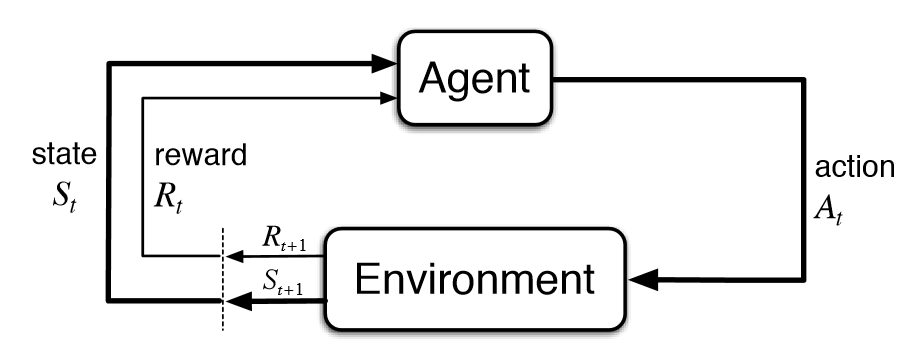
\includegraphics[width=0.8\textwidth]{figures/rl.png}
\caption{\label{fig:RL} Reinforcement Learning Illustration}
\end{figure}


\section{Data set}

TODO

\section{Machine learning methods}

TODO

\section{Design of experiments and performance evaluation}

TODO

% \begin{figure}
% \centering
% \includegraphics[width=0.3\textwidth]{frog.jpg}
% \caption{\label{fig:frog}This frog was uploaded to writeLaTeX via the project menu.}
% \end{figure}


% \begin{thebibliography}{9}
% \bibitem{nano3}
%   K. Grove-Rasmussen og Jesper Nygård,
%   \emph{Kvantefænomener i Nanosystemer}.
%   Niels Bohr Institute \& Nano-Science Center, Københavns Universitet
%
% \end{thebibliography}
\end{document}
